\documentclass[hyperref,UTF8]{ctexart}
    \usepackage[margin=1in]{geometry}
\usepackage{bm}
\usepackage{esvect}
\usepackage{graphicx}
\usepackage{subfigure}
\usepackage{latexsym}
\usepackage{amsfonts}
\usepackage{amssymb}
\usepackage{amsthm}
\usepackage{amssymb}
\usepackage{mhchem}
\usepackage{extpfeil}
\usepackage{hyperref} 
    \newcommand{\zxj}[1]{\bm{#1}$\quad$}
\newcommand{\longequal}{\xlongequal{\quad}}
    \title{``硫''在生活中的存在与运用}
    \author{李夏鲲,邓博以,杨晨阳}
    \date{}
\begin{document}
\maketitle

\section{理论分析与资料概括}

今年暑假,我有幸来到腾冲火山地热公园,参观大自然对人类的一大馈赠——温泉.而那些喷涌出温泉的石缝间,夹杂的是硫的气息.因此,对硫,我渐渐产生了浓厚的兴趣.

在生活中,硫元素处处可见.常见的一个漂白剂就是\ce{SO2};除此之外,厨房的熟客——海波,也叫大苏打,就是硫代硫酸钠;我们的化纤衣服、床单、被套的生产制造也需要用浓硫酸做催化剂;就连我们的身体内部的蛋白质中,甲硫氨酸的存在也让我们感受到了硫元素的亲近.这次,我们小组要找出生活中硫元素的一些存在形式,并通过设计实验了解硫元素的用途,加强我们对硫元素的认识.

提起硫,最先让我们想到的,是厨房里的一种常见物质——硫代硫酸钠.尽管硫代硫酸钠这个名字对于我们可能比较陌生,然而如果说起它的俗称,你就会恍然大悟,原来它就是海波、大苏打啊.在西餐中,大苏打是拿来做面点的重要物质.在工业上,你也别小瞧硫代硫酸钠的功能.它是鞣革时重铬酸盐的还原剂、含氮尾气的中和剂;麦杆和毛的漂白剂以及纸浆漂白时的脱氯剂;它还用于四乙基铅、染料中间体等的制造和矿石提银等.它还是电镀业的还原剂、净水工程的净水剂.在纺织工业中它可用于棉织品漂白后的脱氯剂、染毛织物的硫染剂、靛蓝染料的防白剂、纸浆脱氯剂、医药工业中用作洗涤剂、消毒剂和褪色剂等.养殖业中,它是配置除氯水分析试剂色层分析试剂,点滴分析测定钴、照相定影剂,除氯剂容量分析常用试剂,测定血钠,制备注射液及双糖铁尿素培养基,媒染剂.

为什么硫代硫酸钠用途如此之广?最简单的一个原因,就是它有较强的还原性,而且来源广泛,价格便宜.只要有强氧化性物质的残余,硫代硫酸钠就可以施展它的特长.同时,硫代硫酸钠在分析化学中,可以通过氧化还原滴定测定许多物质的溶液浓度,比如碘液.大苏打还有很强的络合能力,它的水溶液不仅能溶解卤素,还可以和溴化银形成络合物二硫代硫酸合银(I)酸钠\ce{(Na3[Ag(S2O3)2])},因此硫代硫酸钠可以作为定影剂,在洗相片时,过量的大苏打与底片上的未感光部分的溴化银反应,转为可溶的\ce{Na3[Ag(S2O3)2]},把溴化银除掉,使显影部分固定下来.同时,选修四化学教科书上,也指明了硫代硫酸钠在酸性条件下会发生歧化的这一性质.

其次,浓硫酸也是生活中重要的含硫物质之一.大家也许会被浓硫酸可怕的腐蚀性外表所吓到,但是没有了浓硫酸,我们的化纤衣服,床单,涤纶都会不复存在,它是许多有机反应的催化剂.它的强吸水性使它得以成为干燥剂,它的强氧化性与脱水性有时甚至可以作为趣味魔术的秘密.

\ce{SO2}虽然是大气污染气体的一种,但是它的好处却不可被埋没.它有着十分强大的还原性,而且有漂白性.我们的纸张的白净,是二氧化硫用生命谱写的篇章;红酒千年的香醇,是二氧化硫用身躯捍卫的初心.话虽如此,\ce{SO2}还是会严重伤害人体呼吸道,它形成的酸雨也是非常有害的,我们要尽力减少它的危害,发扬它的长处.

最后,硫元素形成的单质硫虽然在日常生活中不易看到,但是它毕竟是硫的单质,几乎所有含硫化工产品,都是直接或间接由硫单质制得.硫单质是硫产品的灵魂.硫单质应用过于广泛,我们就选取了中国古代四大发明——火药,来研究硫单质在里面的作用.

上述的理论分析与资料概括,并不能满足我们探索科学的欲望.下面,我们小组设计了多个实验,身体力行,亲身探索硫与含硫物质的性质.

\section{实验探究}
\subsection{探究硫代硫酸钠的性质}

\subsubsection{大苏打歧化}\label{252.130.196.242}

\zxj{反应原理}\ce{Na2S2O3 + 2HCl $\longequal$ 2NaCl + S v + SO2 ^ + H2O}.

\zxj{实验步骤}取两滴管\ce{Na2S2O3}溶液(图\ref{214.83.84.197})于试管中,加入几滴盐酸,振荡试管,观察实验现象.

\zxj{实验现象}溶液出现黄色浑浊(图\ref{210.21.159.172}),有刺激性气味气体产生.

\zxj{实验结论}大苏打在酸性条件下会歧化,生成硫单质和二氧化硫气体.

\zxj{实验照片}图\ref{206.12.116.92}.

\begin{figure}[h]
    \centering
    \subfigure[\ce{Na2S2O3}溶液]{
        \label{214.83.84.197}
        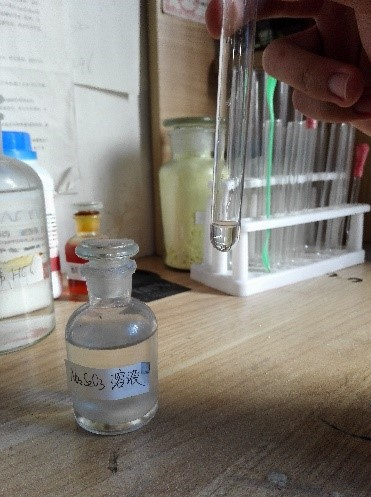
\includegraphics{pic/1.jpg}}
    \hspace{1in}
    \subfigure[黄色沉淀]{
        \label{210.21.159.172}
        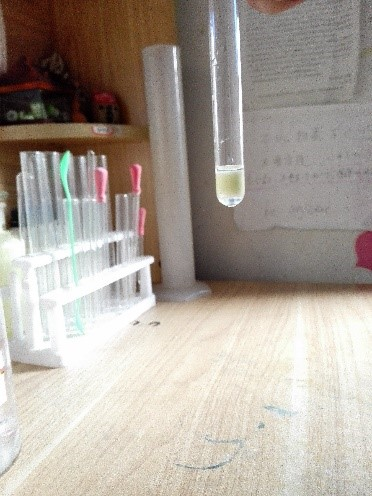
\includegraphics{pic/2.jpg}}
    \caption{\ref{252.130.196.242}的照片}
    \label{206.12.116.92}
\end{figure}

\subsubsection{大苏打还原重铬酸钾}\label{162.233.161.254}

\zxj{反应原理}\ce{3Na2S2O3 + 4K2Cr2O7 + 11H2SO4 \longequal 4Cr2(SO4)3 + 3Na2SO4 + 4K2SO4 + 11H2O}.

\zxj{实验步骤}取两滴管\ce{Na2S2O3}溶液于试管中,加入几滴酸性重铬酸钾溶液(图\ref{230.80.29.124}),振荡试管,观察实验现象.

\zxj{实验现象}酸性重铬酸钾溶液由橙红色变为灰绿色(图\ref{165.182.213.176}).

\zxj{实验结论}大苏打具有还原性,能在酸性条件下将\ce{Cr2O7^2-}还原为\ce{Cr^3+}.

\zxj{实验照片}图\ref{21.229.178.37}.

\begin{figure}[h]
    \centering
    \subfigure[酸性\ce{K2Cr2O7}溶液]{
        \label{230.80.29.124}
        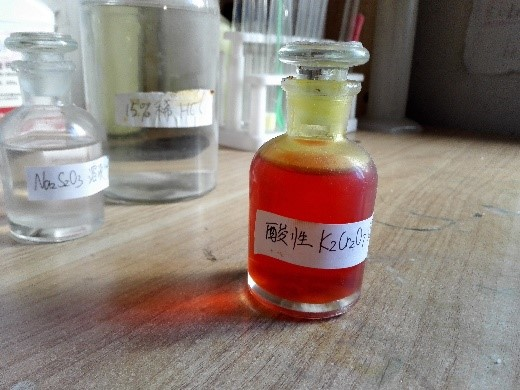
\includegraphics{pic/3.jpg}}
    \hspace{1in}
    \subfigure[溶液变为灰绿色]{
        \label{165.182.213.176}
        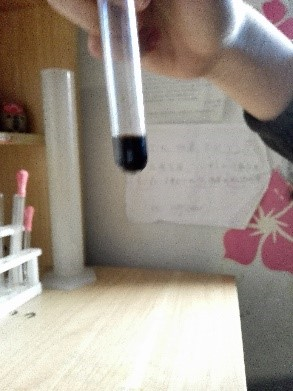
\includegraphics{pic/4.jpg}}
    \caption{\ref{162.233.161.254}的照片}
    \label{21.229.178.37}
\end{figure}

\subsubsection{大苏打使溴水褪色}\label{82.151.94.69}

\zxj{反应原理}\ce{Na2S2O3 + 4Br2 + 5H2O $\longequal$ Na2SO4 + 8HBr + H2SO4}.

\zxj{实验步骤}取少量溴水于试管中,加入几滴硫代硫酸钠溶液,振荡试管,观察实验现象.

\zxj{实验现象}溴水橙色褪去.

\zxj{实验结论}大苏打使\ce{Br2}还原为\ce{Br^-}从而使溴水褪色.

\zxj{实验照片}图\ref{27.158.140.5}.

\begin{figure}[h]
    \centering
    \subfigure[橙色的溴水]{
        \label{89.112.2.237}
        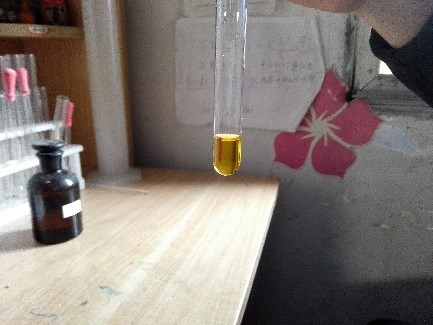
\includegraphics{pic/5.jpg}}
    \hspace{1in}
    \subfigure[溴水褪色]{
        \label{68.194.191.147}
        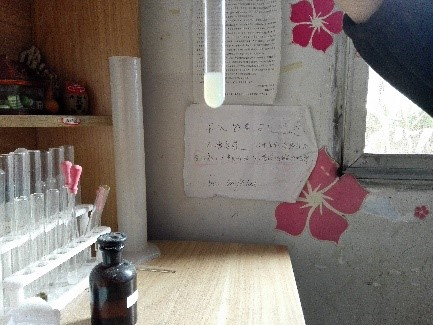
\includegraphics{pic/6.jpg}}
    \caption{\ref{82.151.94.69}的照片}
    \label{27.158.140.5}
\end{figure}

\subsection{探究浓硫酸的性质}

\subsubsection{浓硫酸的脱水性} \label{135.149.167.66}

\zxj{实验原理}浓硫酸具有脱水性,能使纸按照水的氢、氧元素组成比脱去氢、氧而炭化.

\zxj{实验步骤}在玻璃板上放置一张纸巾,在纸巾上滴加两滴浓硫酸,观察纸的
现象.

\zxj{实验现象}滴加浓硫酸处的纸张颜色先变黑后被腐蚀出小洞(图\ref{109.171.91.245}).

\zxj{实验结论}浓硫酸具有脱水性,能使纸张脱水炭化.

\zxj{实验照片}图\ref{254.80.103.3}.

\begin{figure}[h]
    \centering
    \subfigure[纸张被腐蚀出小洞]{
        \label{109.171.91.245}
        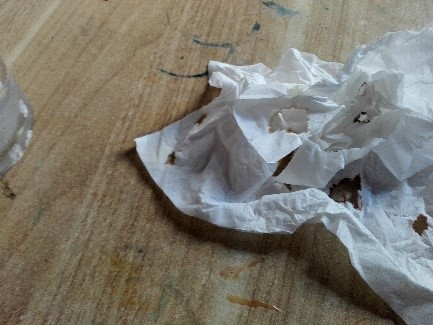
\includegraphics{pic/7.jpg}}
    \caption{\ref{135.149.167.66}的照片}
    \label{254.80.103.3}
\end{figure}

\subsubsection{魔棒点灯实验}\label{158.14.36.238}

\zxj{实验原理}浓硫酸具有强氧化性,与高锰酸钾固体作用会放出大量的热.

\zxj{实验步骤}取少量浓硫酸于试管中,取少量高锰酸钾固体于滤纸上,用玻璃棒一端蘸取少量浓硫酸,然后再蘸取少量高锰酸钾固体,迅速将玻璃棒这端与酒精灯灯芯接触,观察实验现象.

\zxj{实验现象}酒精灯被点燃(图\ref{25.200.140.199}).

\zxj{实验结论}浓硫酸具有强氧化性,与高锰酸钾固体作用会放出大量的热.

\zxj{实验照片}图\ref{157.9.160.83}.

\begin{figure}[h]
    \centering
    \subfigure[酒精灯被点燃]{
        \label{25.200.140.199}
        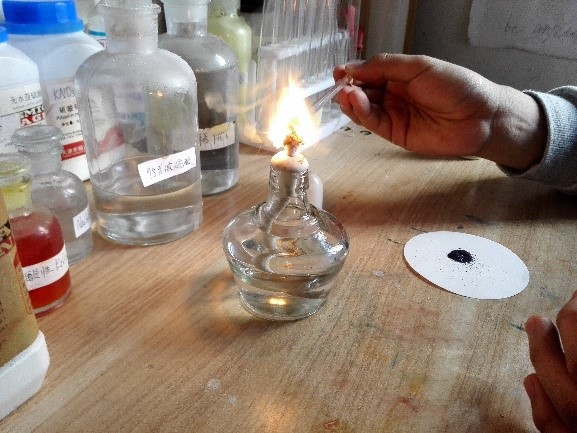
\includegraphics{pic/8.jpg}}
    \caption{\ref{158.14.36.238}的照片}
    \label{157.9.160.83}
\end{figure}

\subsubsection{浓硫酸能催化一些化学反应}\label{73.107.104.102}

\zxj{实验原理}\ce{H2C2O4 $\xlongequal[\Delta]{\textbf{浓硫酸}}$ CO2 ^ + CO ^ + H2O}.

\zxj{实验步骤}按图\ref{250.25.140.131}方式组成实验装置,用排水法收集一瓶CO气体.

\zxj{实验现象}(制取CO时)NaOH洗气瓶外壁温度逐渐升高,草酸不断沸腾(图\ref{96.241.188.81})产生大量气泡;(点燃CO时)产生淡蓝色火焰.

\zxj{实验结论}浓硫酸催化草酸分解产生了CO.

\zxj{实验照片}图\ref{163.71.86.93}.

\begin{figure}[h]
    \centering
    \subfigure[实验装置]{
        \label{250.25.140.131}
        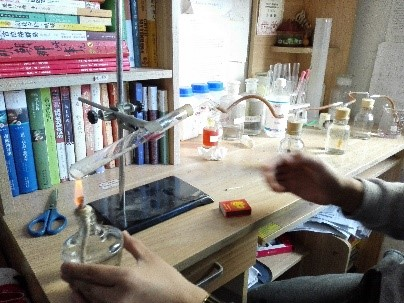
\includegraphics{pic/9.jpg}}
    \hspace{1in}
    \subfigure[草酸不断沸腾]{
        \label{96.241.188.81}
        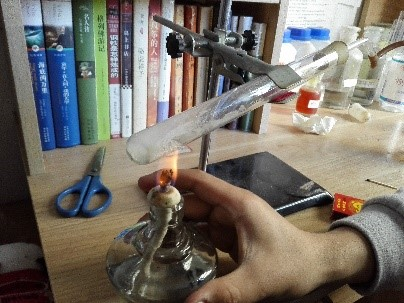
\includegraphics{pic/10.jpg}}
    \caption{\ref{73.107.104.102}的照片}
    \label{163.71.86.93}
\end{figure}

\subsection{硫单质的性质}

\subsubsection{自制黑火药}\label{87.183.133.67}

\zxj{实验原理}\ce{2KNO3 + S + 3C $\xlongequal{点燃}$ K2S + N2 ^ + 3CO2 ^}.

\zxj{实验步骤}上网查阅资料知:黑火药的组成质量比为:硝酸钾75$\%$,碳15$\%$,硫1$\%$.用托盘天平分别称取3g、0.6g、0.4g的硝酸钾、碳粉、硫粉,充分研磨后放入45g规格的彩虹糖塑料筒中,在空旷无人的户外用纸巾将上述粉末混合物在塑料筒中引燃.

\zxj{实验现象}塑料筒发出“砰”的爆炸声,并向外冒出滚滚黑烟,塑料筒熔化.

\zxj{实验结论}自制黑火药成功,黑火药爆炸时能放出大量的热.

\zxj{实验照片}图\ref{89.110.53.22}.

\begin{figure}[h]
    \centering
    \subfigure[黑火药燃烧]{
        \label{250.235.242.84}
        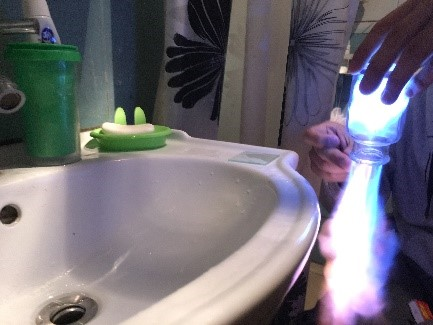
\includegraphics{pic/11.jpg}}
    \hspace{1in}
    \subfigure[黑火药燃烧]{
        \label{155.162.99.152}
        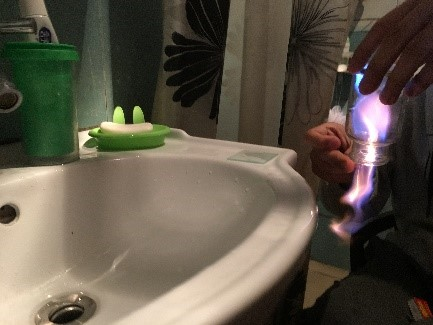
\includegraphics{pic/12.jpg}}
    \caption{\ref{87.183.133.67}的照片}
    \label{89.110.53.22}
\end{figure}

\section{实验活动心得}

\subsection{充分的实验条件}

本次实验活动成功原因之一,在于我们小组组长李夏鲲提供了充分的实验条件,凭借着他丰富的实验经验,在他的领导下,我们妥善处理了遇到的各种特殊情况.

\subsection{化学实验的乐趣}

本次实验活动让我们每个成员都亲身体验了化学实验探究的乐趣,让我们揭开了化学实验神秘的面纱,同时丰富了我们的化学知识,培养了我们的化学兴趣.

\subsection{来自组员邓博以的实验心得体会}

这次研究性学习,我和同学通过实验,一同探究了跟硫即硫的化合物的性质.比如硫代硫酸钠与稀盐酸的反应,硫代硫酸钠与酸性重铬酸钾的反应,浓硫酸催化草酸分解的反应等.虽然我们的实验原理和基本方法来源于教材,可是实际操作与理论知识存在着一定的差异,这就考验我们如何用大脑里的知识解决实际问题,以“魔棒点灯”实验为例,我们在多次“点灯”尝试中,只有一次成功,开始大家认为魔棒温由于度不够,所以无法点燃,但是600摄氏度的高温没有理由点不燃酒精灯,这时,组长李夏鲲同学提出也许是由于浓硫酸有脱水性,将灯芯里的酒精脱水碳化,导致无法点燃,所以我们将灯芯用酒精浸湿后再次实验,果然酒精灯又一次被魔棒点燃.通过这些实验,我们不仅加深对化学知识理解,更锻炼了实践动手能力.

化学是一门与生活息息相关的学科,同时化学实验也是一个探索科学,探索生活的过程.提起化学实验,人们也许会想起因操作不当导致的爆炸,但只要正确操作,合理实验,化学实验不仅不会爆炸(当然,制作黑火药的实验除外),还会拥有无限的魅力.

通过本次活动,我们小组尽可能多地找出生活中硫元素的存在形式,增强对硫元素运用的理解.并且我们小组通过实验亲自了解硫元素的用途,使我们在实验中不仅学习了化学知识,更是培养一种对生活细节的格物致知精神.因此本次活动可谓是圆满成功.

\end{document}